%        File: additional_info.tex
%     Created: Fri Jul 19 04:00 PM 2013 C
% Last Change: Fri Jul 19 04:00 PM 2013 C
%
\documentclass[a4paper]{article}
\usepackage[]{amsmath}
\usepackage[detect-all]{siunitx}
\usepackage{textcomp}
\usepackage{booktabs}
\usepackage[]{graphicx}
\usepackage[utf8]{inputenc} 
\usepackage[T1]{fontenc}
\usepackage[a4paper, bottom=1in]{geometry}
\usepackage{titling}
\usepackage[affil-it]{authblk}
\usepackage[small]{caption}
\usepackage{titlesec}
\usepackage[style=numeric, sorting=none, url=false]{biblatex}
\bibliography{library}

\renewcommand{\bibfont}{\normalfont\small}
\titleformat*{\section}{\normalfont}

\setlength{\droptitle}{-6\baselineskip}   % This is your set screw

\begin{document}
\title{Grating interferometry on a \SI{160}{\kilo\volt} lab source}
\author[1,2]{M. Abis}
\author[1,2]{T. Th\"uring}
\author[2]{Z. Wang}
\author[2]{C. David}
\author[1,2]{M. Stampanoni}
\affil[1]{Institut für Biomedizinische Technik, ETH Z\"urich}
\affil[2]{Swiss Light Source, Paul Scherrer Institut}
\renewcommand{\today}{}
\maketitle
\thispagestyle{empty}

Grating interferometry is an imaging technique that allows the simultaneous
retrieval of attenuation, phase and small angle scattering of X-rays.
It was first demonstrated on synchrotron sources~\cite{David2002}, then
applied to conventional sources with a wide Bremsstrahlung spectrum and low
spatial coherence~\cite{Pfeiffer2006}.

Experiments on lab sources have been performed only for energies
below~\SI{60}{\kilo\eV}, while most applications in medicine and
nondestructive testing require higher penetration power, with voltages
above~\SI{100}{\kilo\V}.
Absorption gratings suitable for high-energy interferometers would then need to be
fabricated with a large thickness and a small pitch, in order to provide
both enough blocking power and sensitivity. The necessary aspect
ratios are thus outside of the reach of the most advanced
microfabrication techniques.

In this presentation, an \emph{edge-on} arrangement of the gratings is
shown~\cite{david2014method}, where the gratings are not illuminated on the face but lay down in
the beam plane, so that arbitrarily high aspect ratios can be achieved at
the cost of one spatial dimension. With such an alignment, it is also easy
to build curved structures that match the beam divergence on short setups.

The design of this kind of setup is shown, as well as the first images taken
with two prototypes with a design energy of~\num{100}
and~\SI{120}{\kilo\eV} realized at PSI~\cite{Thuering2014b}. The short length of the
interferometer, under~\SI{60}{\centi\metre}, makes it also efficient from
the point of view of the flux. The retrieval and meaning of the attenuation,
differential phase and scattering signals is discussed, together with the
possible applications available in this new energy range.

\begin{figure}[h!]
    \centering
    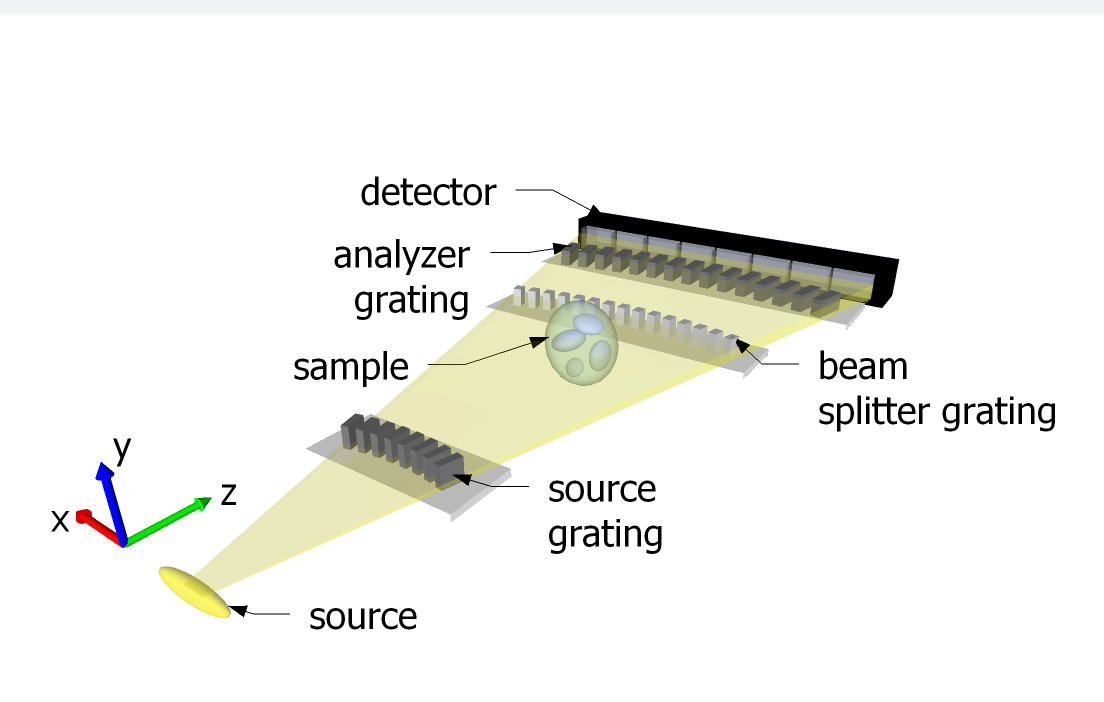
\includegraphics[width=.5\textwidth]{hDPC_setup.png}
    \caption*{Edge-on arrangement for a high-energy interferometer.}\label{fig:edgeon}
\end{figure}
\printbibliography
\end{document}
